% !Mode:: "TeX:DE:UTF-8:Main"
% arara: pdflatex
% arara: pdflatex
% xarara: convert: {density: 160, otheroptions: -dispose previous -delay 10 -loop 0, format: gif}
%magick -density 160 -delay 60 -loop 0 goodbye.pdf goodbye.gif
\PassOptionsToPackage{x11names}{xcolor}

\documentclass{beamer}
\usepackage{tikzlings,tikzducks,xfp}
\usetikzlibrary{overlay-beamer-styles}
\setbeamertemplate{navigation symbols}{}
\definecolor{europablau}{RGB}{00,33,99}
\tikzset{reverseclip/.style={insert path={
(current bounding box.south west) --(current bounding box.north west)
 --(current bounding box.north east) --  (current bounding box.south east)
 -- cycle} }}          
\tikzset{
  bear1/.pic = {
   \begin{scope}[scale=.8,transform shape]
      \bear
  \end{scope}},
  bear2/.pic = {
   \begin{scope}[scale=.6,transform shape]
     \bear;
  \end{scope}},
  bear3/.pic = {
   \begin{scope}[scale=.55,transform shape]
    \bear
  \end{scope}
  },
  bear4/.pic = {\begin{scope}[scale=0.7,transform shape]
  \bear
  \end{scope}
  },
   snowman/.pic = {\begin{scope}[scale=0.7,transform shape]
  \snowman
  \end{scope}
  }
  }
\newcommand\beari{0cm}
\newcommand\bearii{0.3cm}
\newcommand\beariii{0cm}
\newcommand\beariv{0cm}
\newcommand\snowmanh{0.2cm}
\ExplSyntaxOn
\newcommand\myangle[1]{\fpeval{10*sin(#1)}}
\ExplSyntaxOff
\begin{document}
\begin{frame}<1->[plain,label=bears]%%%%%%%%%%%%%%%%%%%%%%%%%%%%%%%%%%%%%%%%%%%%%%%%%
\begin{tikzpicture}[remember picture,overlay]
	
%https://www.motosha.com/wp-content/uploads/old-yellowed-vintage-wallpaper-texture-1024x683.jpg
% Background image
\node[at=(current page.center)]{%
	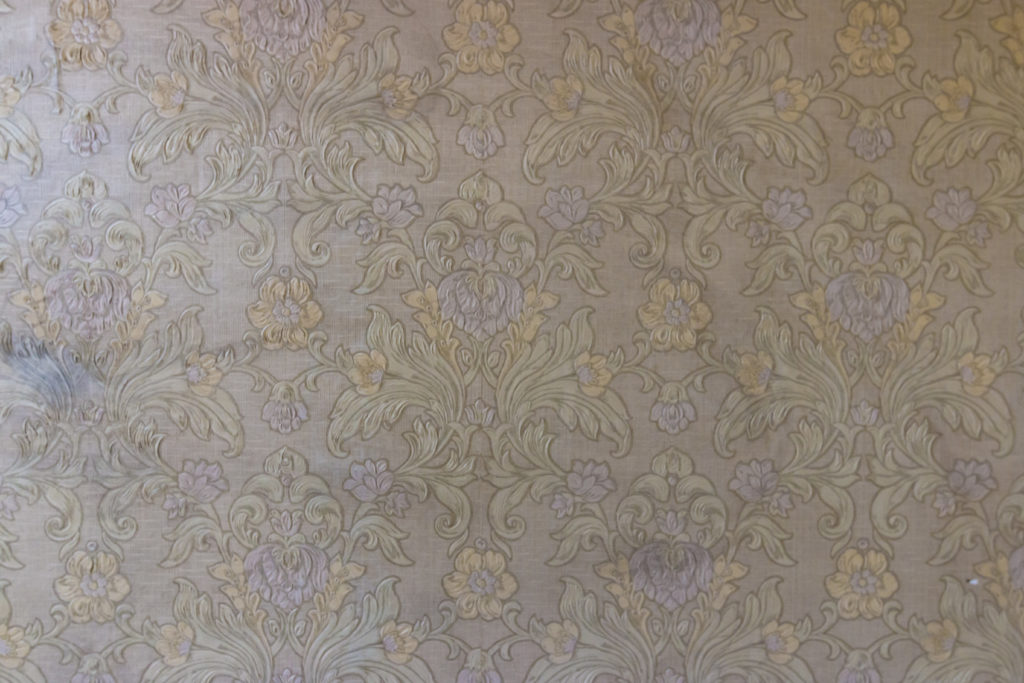
\includegraphics[height=1.05\paperheight]{tapete}
};	

% Image credit of background
\node[at=(current page.south east),xshift=-6.6cm,yshift=0.2cm]{%
	\footnotesize\color{white}};
\end{tikzpicture}

\vspace*{5cm}%\hspace{1cm}
\begin{tikzpicture}[overlay,remember picture]
\fill[brown!60!white!90!blue] ([yshift=+2cm]current page.south west) rectangle (current page.south east);
\end{tikzpicture}%
\begin{tikzpicture}[overlay,shift={(0.5\paperwidth,4cm)}]
   \draw  (-2cm,-0.5cm) coordinate(framebl);
   \draw  (2cm,3cm) coordinate (frametr);
   \fill[Ivory2](framebl) rectangle (frametr);	
   \draw[DarkGoldenrod2!80!black,line width=15pt] (framebl) rectangle (frametr);		
   \draw[brown!60!black,line width=10pt] (framebl) rectangle (frametr);
	%\draw[brown!60!black,line width=10pt] (current page.south east) rectangle (current page.north west);	
  \begin{scope}[scale=1.2,transform shape]
   \bear
   \begin{scope}[even odd rule]

  \clip  (0, 1.55) circle (0.5)[reverseclip];
  \clip  (0.425, 0.3) circle (0.28)[reverseclip];
  \clip  (-0.425, 0.3) circle (0.28)[reverseclip];
  \clip (-1,0.6) --++ (0.45,0)--++(-0.5,1) --cycle[reverseclip] ;
  \clip ( 1,0.6) --++ (-0.45,0)--++(0.5,1) --cycle[reverseclip] ;
  \clip(-1,0.5) rectangle (1,1.2);

  \fill[europablau,rotate around={-50:(0.525,0.9)}](0.525,0.9) ellipse (0.35 and 0.15);
  \fill[europablau,rotate around={50:(-0.525,0.9)}] (-0.525,0.9) ellipse (0.35 and 0.15);
  \fill[europablau] (0,0.75) ellipse (0.55 and 0.65);
  \fill[europablau] (0,0.7) ellipse (0.35 and 0.4);
  \node at (0,0.8){
\includegraphics[width=0.5cm,trim=2cm 0.7cm 2cm 0.7cm,clip]{Flag_of_the_United_Kingdom}};
  \end{scope}
  \end{scope}
\end{tikzpicture}%
\begin{tikzpicture}[scale=1.3,transform shape,baseline={(0,0)}]
 \bear
  \foreach\x in {1,2,...,10}{
  \ifodd\x \only<\x>{
 \fill[draw=brown!30!black,fill=brown,line width=0.4pt] (0.145, 1.38) arc [start angle=-20, end angle=-160, radius=0.16] -- cycle;}\else\only<\x>{} \fi}

 \begin{scope}[even odd rule]

  \clip  (0, 1.55) circle (0.5)[reverseclip];
  \clip  (0.425, 0.3) circle (0.28)[reverseclip];
  \clip  (-0.425, 0.3) circle (0.28)[reverseclip];
  \clip (-1,0.6) --++ (0.45,0)--++(-0.5,1) --cycle[reverseclip] ;
  \clip ( 1,0.6) --++ (-0.45,0)--++(0.5,1) --cycle[reverseclip] ;
  \clip(-1,0.5) rectangle (1,1.2);

  \fill[europablau,rotate around={-50:(0.525,0.9)}](0.525,0.9) ellipse (0.35 and 0.15);
  \fill[europablau,rotate around={50:(-0.525,0.9)}] (-0.525,0.9) ellipse (0.35 and 0.15);
  \fill[europablau] (0,0.75) ellipse (0.55 and 0.65);
  \fill[europablau] (0,0.7) ellipse (0.35 and 0.4);
  \node at (0,0.8){
\includegraphics[width=0.5cm,trim=2cm 0.7cm 2cm 0.7cm,clip]{flag_yellow_eps}};
  \end{scope}
\end{tikzpicture}
%
\begin{tikzpicture}[baseline={(0,0)}]
 \bear
   \foreach\x in {1,2,...,10}{
  \ifodd\x \only<\x>{
 \fill[draw=brown!30!black,fill=brown,line width=0.4pt] (0.145, 1.38) arc [start angle=-20, end angle=-160, radius=0.16] -- cycle;}\else\only<\x>{} \fi}

 \begin{scope}[even odd rule]

  \clip  (0, 1.55) circle (0.5)[reverseclip];
  \clip  (0.425, 0.3) circle (0.28)[reverseclip];
  \clip  (-0.425, 0.3) circle (0.28)[reverseclip];
  \clip (-1,0.6) --++ (0.45,0)--++(-0.5,1) --cycle[reverseclip] ;
  \clip ( 1,0.6) --++ (-0.45,0)--++(0.5,1) --cycle[reverseclip] ;
  \clip(-1,0.5) rectangle (1,1.2);

  \fill[europablau,rotate around={-50:(0.525,0.9)}](0.525,0.9) ellipse (0.35 and 0.15);
  \fill[europablau,rotate around={50:(-0.525,0.9)}] (-0.525,0.9) ellipse (0.35 and 0.15);
  \fill[europablau] (0,0.75) ellipse (0.55 and 0.65);
  \fill[europablau] (0,0.7) ellipse (0.35 and 0.4);
  \node at (0,0.8){
\includegraphics[width=0.5cm,trim=2cm 0.7cm 2cm 0.7cm,clip]{flag_yellow_eps}};
  \end{scope}
\end{tikzpicture}
%
\begin{tikzpicture}[baseline={(0,0)},scale=1.15,transform shape,]
 \bear
   \foreach\x in {1,2,...,10}{
  \ifodd\x \only<\x>{
 \fill[draw=brown!30!black,fill=brown,line width=0.4pt] (0.145, 1.38) arc [start angle=-20, end angle=-160, radius=0.16] -- cycle;}\else\only<\x>{} \fi}
 \begin{scope}[even odd rule]

  \clip  (0, 1.55) circle (0.5)[reverseclip];
  \clip  (0.425, 0.3) circle (0.28)[reverseclip];
  \clip  (-0.425, 0.3) circle (0.28)[reverseclip];
  \clip (-1,0.6) --++ (0.45,0)--++(-0.5,1) --cycle[reverseclip] ;
  \clip ( 1,0.6) --++ (-0.45,0)--++(0.5,1) --cycle[reverseclip] ;
  \clip(-1,0.5) rectangle (1,1.2);

  \fill[europablau,rotate around={-50:(0.525,0.9)}](0.525,0.9) ellipse (0.35 and 0.15);
  \fill[europablau,rotate around={50:(-0.525,0.9)}] (-0.525,0.9) ellipse (0.35 and 0.15);
  \fill[europablau] (0,0.75) ellipse (0.55 and 0.65);
  \fill[europablau] (0,0.7) ellipse (0.35 and 0.4);
  \node at (0,0.8){
\includegraphics[width=0.5cm,trim=2cm 0.7cm 2cm 0.7cm,clip]{flag_yellow_eps}};
  \end{scope}
\end{tikzpicture}
%
\includegraphics{tartan}
\begin{tikzpicture}[baseline={(0,0)}]
 \bear
   \foreach\x in {1,2,...,10}{
  \ifodd\x \only<\x>{
 \fill[draw=brown!30!black,fill=brown,line width=0.4pt] (0.145, 1.38) arc [start angle=-20, end angle=-160, radius=0.16] -- cycle;}\else\only<\x>{} \fi}
 \begin{scope}[even odd rule]

  \clip  (0, 1.55) circle (0.5)[reverseclip];
  \clip  (0.425, 0.3) circle (0.28)[reverseclip];
  \clip  (-0.425, 0.3) circle (0.28)[reverseclip];
  \clip (-1,0.6) --++ (0.45,0)--++(-0.5,1) --cycle[reverseclip] ;
  \clip ( 1,0.6) --++ (-0.45,0)--++(0.5,1) --cycle[reverseclip] ;
  \clip(-1,0.5) rectangle (1,1.2);

  \fill[europablau,rotate around={-50:(0.525,0.9)}](0.525,0.9) ellipse (0.35 and 0.15);
  \fill[europablau,rotate around={50:(-0.525,0.9)}] (-0.525,0.9) ellipse (0.35 and 0.15);
  \fill[europablau] (0,0.75) ellipse (0.55 and 0.65);
  \fill[europablau] (0,0.7) ellipse (0.35 and 0.4);
  \node at (0,0.8){
\includegraphics[width=0.5cm,trim=2cm 0.7cm 2cm 0.7cm,clip]{flag_yellow_eps}};
  \end{scope}
\end{tikzpicture}


%\begin{tikzpicture}[remember picture, overlay]
%\node at ({5.4+0.1*sin(\thepage)},{31.16-0.0472*(\thepage)}) {
\includegraphics[width=\paperwidth]{snowflakes}};
%\end{tikzpicture}

\end{frame}
\end{document} 